\thispagestyle{empty}
\BgThispage
\begin{center}
    \LARGE
    \textbf{Software Requirements Specification \\
    (Спецификация требований к продукту)} \\
    \normalsize
\end{center}

\begin{enumerate}
    \item \textbf{Introduction (Введение)}
    \begin{enumerate}[label=1.\arabic*]
        \item Purpose \\
        Цель документа заключается в определении требований к реализуемому продукту, используемых технологий,
        методологий и накладываемых ограничений. Описание процесса разработки и эксплуатирования с возможными издержками.
        \item Scope (Область применения) \\
        Данный документ относится к проекту ``Эхо Петербурга'' - сетевому партнеру радиостанции ``Эхо Москвы''. Документ
        создан для использования разработчиками, дизайнерами, тестировщиками, заказчиками
        \item Definitions, Acronyms and Abbreviations (Определения и аббревиатуры) \\
        JavaScript - язык программирования, который используют разработчики для создания интерактивных веб-страниц. \\
        PHP - язык программирования общего назначения, интенсивно применяемый для разработки веб-приложений. \\
        TCP/IP - сетевая модель передачи данных, представленных в цифровом виде. \\
        API - (интерфейс прикладного программирования) - это набор определенных правил, которые позволяют различным приложениям взаимодействовать друг с другом. \\
        Внедрение SQL-кода - один из распространённых способов взлома сайтов и программ, работающих с базами данных, основанный на внедрении в запрос произвольного SQL-кода. \\
        Внедрение HTML-кода - способ взлома сайтов и программ, путём ручного редактирования кода элемента страницы. \\
        Cookie (куки) - небольшой фрагмент данных, отправленный веб-сервером и хранимый на компьютере пользователя.\\
        Backup (бэкап) - процесс создания копии данных на носителе (жёстком диске, дискете и т. д.), предназначенном для восстановления данных в оригинальном или новом месте их расположения в случае их повреждения или разрушения. \\
        Front-end (фронтенд) - презентационная часть информационной или программной системы, её пользовательский интерфейс и связанные с ним компоненты (та часть, что видит пользователь). \\
        Interface (интерфейс) - совокупность средств, методов и правил взаимодействия (управления, контроля и т. д.) между элементами системы. \\
        User Interface (пользовательский интерфейс) - интерфейс, обеспечивающий передачу информации между пользователем-человеком и программно-аппаратными компонентами котьютерной системы. \\
        DoS (Denial of Service ``отказ в обслуживании'') - хакерская атака на вычислительную систему с целью довести её до отказа. \\
        DDoS - DoS атака, выполняющаяся одновременно с большого числа компьютеров. \\
        Превью новости - это краткое изложение основной информации, которая будет описана в статье. \\
        Топ — рейтинг объектов, упорядоченных в порядке убывания по определённому критерию. \\
        Топ-N новостей - N верхних позиций топа новостей по популярности, где (N - натуральное число) \\
        ПК - персональный компьютер \\
        Тег - метка, использующаяся для классификации или описания объектов, данных или информации в различных контекстах. \\
        Баг - это ошибка, дефект или неисправность в программном обеспечении или веб-сайте.\\
        RESTful API (Representational State Transfer) — это архитектурный стиль для создания веб-сервисов, основанный на
        протоколе HTTP. RESTful API использует HTTP-методы, такие как GET, POST, PUT и DELETE, для передачи данных и
        выполняет операции с ресурсами. \\
        Принципы RESTful API включают в себя:\\
        \quad Основной принцип RESTful API состоит в том, что каждый ресурс (например, пользователь, сообщение или
        изображение) должен иметь уникальный идентификатор (URI), который позволяет обращаться к нему через
        HTTP-методы, такие как GET, POST, PUT и DELETE.\\
        \quad Ограничение клиент-сервер: веб-сервер должен быть независимым от клиента, чтобы обеспечить масштабируемость
        и упрощение архитектуры.\\
        \quad Без состояния (stateless): каждый запрос клиента должен содержать все необходимые данные для выполнения
        запроса, чтобы сервер не хранил информацию о состоянии клиента.
        \item References (Ссылки) \\
        \url{https://echomsk.spb.ru}  - главный домен сервиса
        \item Overview (Обзор документа) \\
        Общее описание - Данный раздел содержит описание факторов, влияющих на требования к продукту, сами требования
        описываются в следующем разделе. \\
        Спецификация требований - Данный раздел содержит описание всех требований к разрабатываемой системе. Данное
        описание будет использоваться как разработчиками при разработке системы, так и тестировщиками в процессе проверки ее функционала.
    \end{enumerate}
    \BgThispage
    \item \textbf{Overall Description (Общее описание)}
    \begin{enumerate}[label=2.\arabic*]
        \item Product functions (Функциональность продукта) \\
        ``Эхо Петербурга'' - это сетевое издание, которое предоставляет точную, оперативную и полную информации в
        виде новостей или статистики 24 часа в сутки 7 дней в неделю.
        \item User characteristics (Описание пользователей) \\
        Посетители сайта ( читатели ) - это люди, которые переходят на сайт ``Эхо Петербурга'' в браузере, ищут и
        читают новости и статистику по Covid-19, делятся новостями в соц.сетях и переходят на сайты-источники новостей. \\
        Администратор новостного сайта – это пользователь с расширенными правами, которые позволяют ему управлять содержанием и настройками сайта.
        Он имеет доступ к административной панели сайта с локального сервера, где может управлять различными параметрами сайта.
        \item Assumptions and dependencies (Влияющие факторы и зависимости) \\
        В системе различные функциональные компоненты системы должны быть выделены в отдельные модули, такие как база
        данных, сервер приложений и веб-сервер. \\
        Система должна быть способна к созданию резервных копий модулей, таких как база данных и сервер приложений, и
        перенаправлять запросы к этим копиям в случае отключения основных модулей. \\
        Система должна использовать методы балансировки нагрузки, такие как кластеризация, для распределения запросов
        между различными модулями. \\
        Система должна содержать функционал для тестирования и мониторинга ее компонентов, чтобы быстро обнаруживать
        проблемы и устранять их. Например, система может использовать мониторинг производительности, для анализа
        использования ресурсов сервера, и автоматический тестировщик, для проверки функциональности сайта после внесения изменений. \\
        Система должна поддерживать \\
        \quad Операционные системы:
        \begin{itemize}
            \item Windows 10 или более поздние версии
            \item macOS X 10.14 или более поздние версии
            \item iOS 13 или более поздние версии для мобильных устройств Apple
            \item Android 8.0 или более поздние версии для мобильных устройств Android
        \end{itemize}
        \quad Браузеры:
        \begin{itemize}
            \item Google Chrome версии 111.0.5563
            \item Mozilla Firefox версии 111.0
            \item Apple Safari версии 14.1.2
            \item Microsoft Edge версии 111.0.1661
            \item Opera версии 96.0.4693
        \end{itemize}
        \quad Дополнительные требования к браузерам:
        \begin{itemize}
            \item Поддержка HTML5, CSS3, JavaScript
            \item Поддержка медиа-контента, такого как изображения
            \item Поддержка HTTPS для защиты данных пользователей
        \end{itemize}
        \item Сonstraints (Ограничения) \\
        Портал не предусматривает аутентификацию пользователей.
    \end{enumerate}
    \BgThispage
    \item \textbf{Specific Requirements (Спецификация требований)}
    \begin{enumerate}[label=3.\arabic*]
        \item Functionality (Функциональные требования)
        \begin{enumerate}[label=3.1.\arabic*]
            \item Система должна предоставлять пользователю информацию в виде новостей в форме превью с возможностю перейти к расширенному взаимодействию с новостью.
            \item Система должна собирать статистику по просмотру новостей.
            \item Система должна предоставлять пользователю возможность выполнять поиск новостей по тегам.
            \item Система должна предоставлять пользователю возможность выполнять поиск по совпадению слов в новостях.
            \item Система должна предоставлять пользователю возможность выполнять фильтрацию новостей по категориям.
            \item Система должна предоставлять пользователю возможность поделиться новостью в соц. сетях.
            \item Система должна предоставлять пользователю возможность перейти к источнику новости.
            \item Система должна предоставлять пользователю возможность просматривать ежедневно обновляемую статистику по заболеваемости COVID-19
            \item Система должна предоставлять пользователю возможность оставить обратную связь.
            \item Администратор должен иметь возможность войти в систему административного доступа на локальном сервере с помощью логина и пароля.
            \item Система должна проверять и аутентифицировать учетные данные администратора перед предоставлением доступа к административной панели сайта.
            \item Система должна предоставлять администратору возможность добавлять, редактировать и удалять новости на сайте.
            \item Система должна предоставлять администратору возможность добавление новости, включающее в себя заполнение
            необходимых полей, таких как заголовок, категория, теги, изображение, содержание новости и ссылки на источник.
            \item Система должна предоставлять администратору возможность редактировать или удалять любую новость на сайте.
            \item Система должна предоставлять администратору возможность просматривать статистику посещений сайта, такую как количество уникальных посетителей, просмотры страниц.
        \end{enumerate}
        \BgThispage
        \item Usability (Требования к удобству использования)
        \begin{enumerate}[label=3.2.\arabic*]
            \item В пользовательском интерфейсе системы должны быть вынесены отдельно тематики новостей и выделены графически.
            \item В пользовательском интерфейсе системы на главной странице должны быть вынесены отдельно топ-4 новости.
            \item В пользовательском интерфейсе системы на главной странице должны быть вынесены отдельно топ-20 тегов и выделены графически.
            \item Страница должна в среднем прогружаться за 2-5 секунд при интернет-соединении 100 Мбит/сек для комфортного восприятия
            пользователями с различным опытом использования ПК.
            \item В пользовательском интерфейсе системы должна отсутствовать реклама.
        \end{enumerate}
        \newpage
        \item Reliability (Требования к надежности)
        \begin{enumerate}[label=3.3.\arabic*]
            \item Cистема должна работать без перебоев 24/7, не считая часы профилактики.
            \item В системе необходимо будет определить часы профилактики, направленные на поддержание работоспособности,
            внедрение обновлений, исправление багов, длительностью не более двух часов еженедельно во временном
            интервале с самой низкой активностью пользователей, на основании анализа статистики, собранной в течение
            первого месяца работы системы. В течение первого месяца часы профилактики определены с 02 до 04 часов каждый понедельник,
            как предположительные часы с самой низкой активностью пользователей. В дальнейшем часы профилакткии могут быть пересмотрены,
            исходя из анализа статистики за полугодие.
            \item В случае непредвиденной критической ошибки система должна восстанавливаться и загружаться из бэкапа не более чем за 3 минуты, запускаться не более чем 10 минут.
            \item Система должна обладать защитой от DOS и DDOS атак.
            \item Система должна обладать защитой от sql-внедрений.
            \item Система должна обладать защитой от html-внедрений.
%            \item Система должна стабильно функционировать при резком наплыве пользователей (х2 от предполагаемой нагрузки в 5 тыс. одновременных пользователей).
        \end{enumerate}
        \item Performance (Требования к производительности)
        \begin{enumerate}[label=3.4.\arabic*]
            \item Система должна отвечать на запросы пользователя не дольше 5 секунд при интернет-соединении 100 Мбит/сек.
            \item Система должна иметь среднее время ответа 3 секунды при интернет-соединении 100 Мбит/сек.
            \item Система должна стабильно обрабатывать 200 транзакций в секунду. \\
            \tiny \textit{(2 млн жителей ленобласти - 300 тыс. детей, из них 10\% заходит на сайт, /24/60/60 секунд и *50 средних запросов в день *2 для надёжности)}
            \normalsize
            \item Система должна стабильно одновременно обслуживать 5000 пользователей.
            \tiny \textit{(один запрос в среднем раз в 20 секунд, +1000 для надёжности)}
            \normalsize
        \end{enumerate}
        \item Design Constraints (Ограничения разработки) \\
        Система должна иметь адаптивную вёрстку. \\
        Во front-end части системы должен использоваться JavaScript стандарта ECMAScript 2022. \\
        В серверной части системы должен использоваться PHP версии 8.1 для обработки запросов пользователей.
        \item Interfaces (Интерфейсы)
        \BgThispage
        \begin{enumerate}[label=3.6.\arabic*]
            \item User Interfaces (Пользовательские интерфейсы): \\
            На главной странице сайта гость видит шапку, содержащую логотип, поиск и кнопку с выпадающим меню.
            Выпадающее меню появляется слева и содержит навигацию по сайту. По центру главной страницы
            располагается главная новость дня, занимающая 50\% пространства по вертикали. Сбоку от главной
            новости располагается топ новостей. Под главной новостью расположены ссылки на отфильтрованные
            новости по тегам.В нижней части страницы расположены превью всех новостей за данный день, отсортированные
            по времени добавления. Превью новостей содержат дату и время добавления, название новости, изображение и начало новости. \\
            Страница со статистикой Covid-19 содержит таблицу с числом заболевших, выздоровевших и умерших от covid-19 за текущие сутки. \\
            На странице ``Контакты'' расположена форма для обратной связи, содержащая поля для записи почты, имени и сообщения, а также кнопку ``отправить''. Под формой расположена информация о редакции и о команде проекта. \\
            На странице ``Политика конфиденциальности'' находится положение о COOKIE и обработке персональных данных. \\
            На странице ``Соглашение'' расположены Правила использования материалов сайта echomsk.spb.ru .
            \item Hardware Interfaces (Аппаратные интерфейсы): \\
            64gb ram. \\
            2 xeon 64 ядер 3.0 GHz. \\
            2 ТБ на все необходимое ПО, бэкап сервисы, память под сам бэкап etc. \\
            Системные требования для серверной машины выбраны с учётом предъявленных требований к надёжности и стабильности системы,
            а так же с запасными мощностями для стабильной работы при непредвиденных нагрузках и дальнейшего возможного расширения проекта.
            \item Software Interfaces (Программные интерфейсы): \\
            API Facebook/Twitter/VK/Pinterest/reddit content publishing
            \item Communications Interfaces (Сетевые интерфейсы): \\
            RESTful API: RESTful API предоставляет простой и гибкий интерфейс для взаимодействия с новостным сайтом.
            Он может быть использован для получения списка новостей, поиска новостей по ключевым словам или категориям,
            создания, редактирования и удаления новостей.\\
        \end{enumerate}
        \item Licensing Requirements (Требования к лицензированию) \\
        \BgThispage
        Лицензия сетевого издания реестра зарегистрированных СМИ (ФС77 - 38973) (( истек , иностранный агент)) \\
        Система распространяется под проприетарной лицензией. Раскрытие и использование исходных кодов программ и прочих компонентов системы разрешается исключительно с письменного согласия владельцев продукта.
    \end{enumerate}
\end{enumerate}
\newpage
\BgThispage
\begin{center}
    \large
    \textbf{Атрибуты функциональных \\ требований\\}
    \small
    \begin{tabular}{|c|c|c|c|c|}
        \hline
        N\textsuperscript{\underline{o}} & Требование                    & Приоритетность & Чел./ч & Риски*  \\
        \hline
        1                                & Предоставление новостей       & Критическая    & 8      & Низкие  \\
        \hline
        2                                & Cбор статистики по просмотрам & Средняя        & 8      & Низкие  \\
        \hline
        3                                & Поиск по тегам                & Низкая         & 6      & Низкие  \\
        \hline
        4                                & Поиск по совпадающим словам   & Низкая         & 4      & Низкие  \\
        \hline
        5                                & Фильтрация по категориям      & Низкая         & 4      & Низкие  \\
        \hline
        6                                & Переход от превью к           & Высокая        & 4      & Средние \\
        & расширенной новости           &                &        &         \\
        \hline
        7                                & Sharing в соц. сети           & Средняя        & 6      & Высокие \\
        \hline
        8                                & Переход к источнику новости   & Критическая    & 2      & Высокие \\
        \hline
        9                                & Статистика по COVID-19        & Высокая        & 6      & Средние \\
        \hline
        10                               & Возможность обратной связи    & Средняя        & 4      & Низкие  \\
        \hline
    \end{tabular}
\end{center}
\large
\begin{center}
    \textbf{Атрибуты нефункциональных требований\\}
\end{center}
\begin{center}
    \small
    \begin{tabular}{|c|c|c|c|c|}
        \hline
        N\textsuperscript{\underline{o}} & Требование                      & Приоритетность & Чел./ч & Риски*  \\
        \hline
        1                                & Выделить топ новостей           & Высокая        & 4      & Высокие \\
        \hline
        2                                & Загрузка страницы за 2-5 сек    & Критическая    & 8      & Высокие \\
        \hline
        3                                & Отсутсвие рекламы               & Высокая        & 0      & Низкие  \\
        \hline
        4                                & Стабильная работа системы       & Критическая    & 16     & Высокие \\
        \hline
        5                                & Защита от хакеров               & Высокая        & 30     & Средние \\
        \hline
        6                                & Обработка ~200 транзакций/сек   & Высокая        & 16     & Средние \\
        \hline
        7                                & Оптимизация памяти пользователя & Средняя        & 12     & Высокие \\
        \hline
        8                                & Адаптивная вёрстка              & Критическая    & 6      & Низкие  \\
        \hline
    \end{tabular}\\

\end{center}
\vspace{0.5cm}
\begin{center}
    \large
    \textbf{Пояснения к рискам.}\\
\end{center}
\normalsize
\textit{Функциональные:}
\begin{enumerate}[noitemsep,topsep=0pt,parsep=0pt,partopsep=0pt]
    \item довольно стабильный процесс с низким шансом возникновения неожиданностей.
    \item используется простое и стабильное API.
    \item используется простой и предсказуемый алгоритм.
    \item используется простой и предсказуемый алгоритм.
    \item используется простой и предсказуемый алгоритм.
    \item возможен переход на несуществующую страницу из-за некорректного составления новости или истечения срока действия страницы.
    \item используется множество API, стабильность работы которых зависит от их разработчиков.
    \item возможен переход на несуществующую страницу из-за непредсказуемого поведения источника.
    \item используется чужое API, стабильность которого зависит от разработчика.
    \item предсказуемая функция с простой реализацией.
\end{enumerate}
\newpage
\BgThispage
\textit{Нефункциональные:}
\begin{enumerate}[noitemsep,topsep=0pt,parsep=0pt,partopsep=0pt]
    \item необходимо рассмотреть краевые случаи по приоритезации новостей и их корректное отображение.
    \item по умолчанию страницы легковесные, загрузка за подобное время сопровождается доп. нагрузкой на сеть или ожиданием, что может повлечь чрезмерную нагрузку на сервер в случае большого наплыва пользователей.
    \item отсутствие доп. дохода.
    \item Клименков С.В. : “Чем сильнее мы пытаемся повысить надежность системы, тем менее стабильно она работает”.
    \item передача внутреннего доступа и делегирование обязанностей сторонним лицам ( компаниям ).
    \item увеличение производительности влечет за собой доп. риски по стабильности системы.
    \item влечет увеличение использование памяти на стороне сервера и вытекающие из этого риски.
    \item простая функция, реализация которой давно изучена и используется во всех крупных проектах, имеет предсказуемый результат.
\end{enumerate}
\begin{center}
    \large
    \textbf{Прецеденты\\}
    \small
    \begin{tabular}{|l|l|}
        \hline
        Имя                   & Искать новость                                \\
        \hline
        ID                    & 1                                             \\
        \hline
        Описание              & Пользователь сайта осуществляет поиск новости \\
        \hline
        Актеры                & Пользователь                                  \\
        \hline
        Основной поток        & Пользователь выбирает инструмент для поиска,  \\
        & ищет новость и выбирает интересующую          \\
        \hline
        Постусловия           & -                                             \\
        \hline
        Альтернативные потоки & -                                             \\
        \hline
    \end{tabular}\\
    \vspace{0.5cm}
    \begin{tabular}{|l|l|}
        \hline
        Имя                   & Искать новость по тегам                        \\
        \hline
        ID                    & 2                                              \\
        \hline
        Описание              & Пользователь сайта осуществляет поиск новости, \\
        & выбирая нужный тег                             \\
        \hline
        Актеры                & Пользователь                                   \\
        \hline
        Основной поток        & Пользователь выбирает нужный тег,              \\
        & нажимает на него, скроллит страницу с          \\
        & новостями и выбирает интересующую              \\
        \hline
        Постусловия           & -                                              \\
        \hline
        Альтернативные потоки & -                                              \\
        \hline
    \end{tabular}\\
    \vspace{0.5cm}
    \begin{tabular}{|l|l|}
        \hline
        Имя                   & Искать новость в поисковой строке              \\
        \hline
        ID                    & 3                                              \\
        \hline
        Описание              & Пользователь сайта осуществляет поиск          \\
        & новости в поисковой строке                     \\
        \hline
        Актеры                & Пользователь                                   \\
        \hline
        Основной поток        & Пользователь нажимает на значок поиска, вводит \\
        & название новости или ключевые слова и выбирает \\
        & интересующую новость из результата поиска      \\
        \hline
        Постусловия           & -                                              \\
        \hline
        Альтернативные потоки & -                                              \\
        \hline
    \end{tabular}
\end{center}

\newpage
\BgThispage
1000-7?
\begin{center}
    \small
    \begin{tabular}{|l|l|}
        \hline
        Имя                   & Искать новость по темам                             \\
        \hline
        ID                    & 4                                                   \\
        \hline
        Описание              & Пользователь сайта осуществляет поиск новости,      \\
        & выбирая нужную тему                                 \\
        \hline
        Актеры                & Пользователь                                        \\
        \hline
        Основной поток        & Пользователь выбирает нужную тему в шапке страницы, \\
        & нажимает на него, скроллит страницу                 \\
        & с новостями и выбирает интересующую                 \\
        \hline
        Постусловия           & -                                                   \\
        \hline
        Альтернативные потоки & -                                                   \\
        \hline
    \end{tabular}\\
    \vspace{0.5cm}
    \begin{tabular}{|l|l|}
        \hline
        Имя                   & Искать новость по темам                      \\
        \hline
        ID                    & 5                                            \\
        \hline
        Описание              & Пользователь открывает выбранную на сайте    \\
        & новость и читает ее                          \\
        \hline
        Актеры                & Пользователь                                 \\
        \hline
        Основной поток        & Пользователь нажимает на заголовок выбранной \\
        & новости, открывается полная                  \\
        & версия, гость читает ее                      \\
        \hline
        Постусловия           & -                                            \\
        \hline
        Альтернативные потоки & Делится новостью                             \\
        & Переходит к источнику новости                \\
        \hline
    \end{tabular}\\
    \vspace{0.5cm}
    \begin{tabular}{|l|l|}
        \hline
        Имя                   & Поделиться новостью                        \\
        \hline
        ID                    & 6                                          \\
        \hline
        Описание              & Пользователь делится новостью в соц. сетях \\
        \hline
        Актеры                & Пользователь                               \\
        \hline
        Основной поток        & Пользователь нажимает на кнопку            \\
        & "поделиться" нужной соц.сети               \\
        \hline
        Постусловия           & Ссылка на новость отправлена               \\
        \hline
        Альтернативные потоки & -                                          \\
        \hline
    \end{tabular}\\
    \vspace{0.8cm}
    \begin{tabular}{|l|l|}
        \hline
        Имя                   & Перейти к источнику новости                           \\
        \hline
        ID                    & 7                                                     \\
        \hline
        Описание              & Пользователь осуществляет переход с источнику новости \\
        \hline
        Актеры                & Пользователь                                          \\
        \hline
        Основной поток        & Пользователь нажимает на кнопку “источник”,           \\
        & после чего осуществляется редирект на статью-источник \\
        \hline
        Постусловия           & Осуществлен редирект на статью на сайте-источнике     \\
        \hline
        Альтернативные потоки & -                                                     \\
        \hline
    \end{tabular}
\end{center}
\newpage
\BgThispage
\begin{flushright}
    \mbox{сожрать сожрать сожрать сожрать сожрать сожрать сожрать сожрать сожрать сожрать сожрать сожрать сожрать сожрать сожрать сожрать сожрать сожрать сожрать сожрать сожрать сожрать сожрать сожрать сожрать сожрать сожрать сожрать}
\end{flushright}
\begin{center}
    \small
    \begin{tabular}{|l|l|}
        \hline
        Имя                   & Смореть Covid-статистику                        \\
        \hline
        ID                    & 8                                               \\
        \hline
        Описание              & Пользователь открывает статистику и смотрит ее  \\
        \hline
        Актеры                & Пользователь                                    \\
        \hline
        Основной поток        & Пользователь нажимает на кнопку Covid-19,       \\
        & осуществляется переход к странице с таблицей,   \\
        & пользователь смотрит статистику за текущую дату \\
        \hline
        Постусловия           & -                                               \\
        \hline
        Альтернативные потоки & -                                               \\
        \hline
    \end{tabular}\\
    \vspace{0.5cm}
    \begin{tabular}{|l|l|}
        \hline
        Имя                   & Отправить обратную связь                                    \\
        \hline
        ID                    & 9                                                           \\
        \hline
        Описание              & Пользователь заполняет форму обратной связи и отправляет ее \\
        \hline
        Актеры                & Пользователь                                                \\
        \hline
        Основной поток        & Пользователь нажимает на кнопку Контакты, осуществляется    \\
        & переход к странице с формой для обратной связи,             \\
        & заполняет ее и нажимает кнопку “отправить”.                 \\
        \hline
        Постусловия           & Обратная связь отправлена                                   \\
        \hline
        Альтернативные потоки & -                                                           \\
        \hline
    \end{tabular}\\
    \vspace{0.5cm}
    \begin{tabular}{|l|l|}
        \hline
        Имя                   & Авторизоваться в системе                                      \\
        \hline
        ID                    & 10                                                            \\
        \hline
        Описание              & Администратор пытается авторизоваться                         \\
        \hline
        Актеры                & Администратор                                                 \\
        \hline
        Основной поток        & Администратор сайта вводит необходимые данные для авторизации \\
        \hline
        Постусловия           & Получен доступ к функционалу администратора                   \\
        \hline
        Альтернативные потоки & Отказано в доступе                                            \\
        \hline
    \end{tabular}\\
    \vspace{0.5cm}
    \begin{tabular}{|l|l|}
        \hline
        Имя                   & Добавить новость                              \\
        \hline
        ID                    & 11                                            \\
        \hline
        Описание              & Администратор доавляет новость на сайт        \\
        \hline
        Актеры                & Администратор                                 \\
        \hline
        Основной поток        & Администратор сайта вводит необходимые данные \\
        & новости, ссылки, отмечает тематику новости    \\
        \hline
        Постусловия           & Добавлена новость на сайт                     \\
        \hline
        Альтернативные потоки & -                                             \\
        \hline
    \end{tabular}\\
\end{center}
\newpage
\BgThispage
\begin{center}
\begin{tabular}{|l|l|}
    \hline
    Имя                   & Редактировать новость                        \\
    \hline
    ID                    & 12                                           \\
    \hline
    Описание              & Администратор редактирует новость с сайта    \\
    \hline
    Актеры                & Администратор                                \\
    \hline
    Основной поток        & Администратор сайта ищет необходимую новость \\
    & и изменяет все необходимые данные            \\
    \hline
    Постусловия           & Новость изменена                             \\
    \hline
    Альтернативные потоки & -                                            \\
    \hline
\end{tabular}\\
\vspace{0.8cm}
\begin{tabular}{|l|l|}
    \hline
    Имя                   & Удалить новость                                           \\
    \hline
    ID                    & 13                                                        \\
    \hline
    Описание              & Администратор удаляет новость с сайта                     \\
    \hline
    Актеры                & Администратор                                             \\
    \hline
    Основной поток        & Администратор сайта ищет необходимую новость и удаляет ее \\
    \hline
    Постусловия           & Новость удалена с сайта                                   \\
    \hline
    Альтернативные потоки & -                                                         \\
    \hline
\end{tabular}\\
\end{center}
\begin{center}
    \LARGE
    \textbf{UML-usecases}
    \normalsize
        \begin{figure}[H]
        \centering
        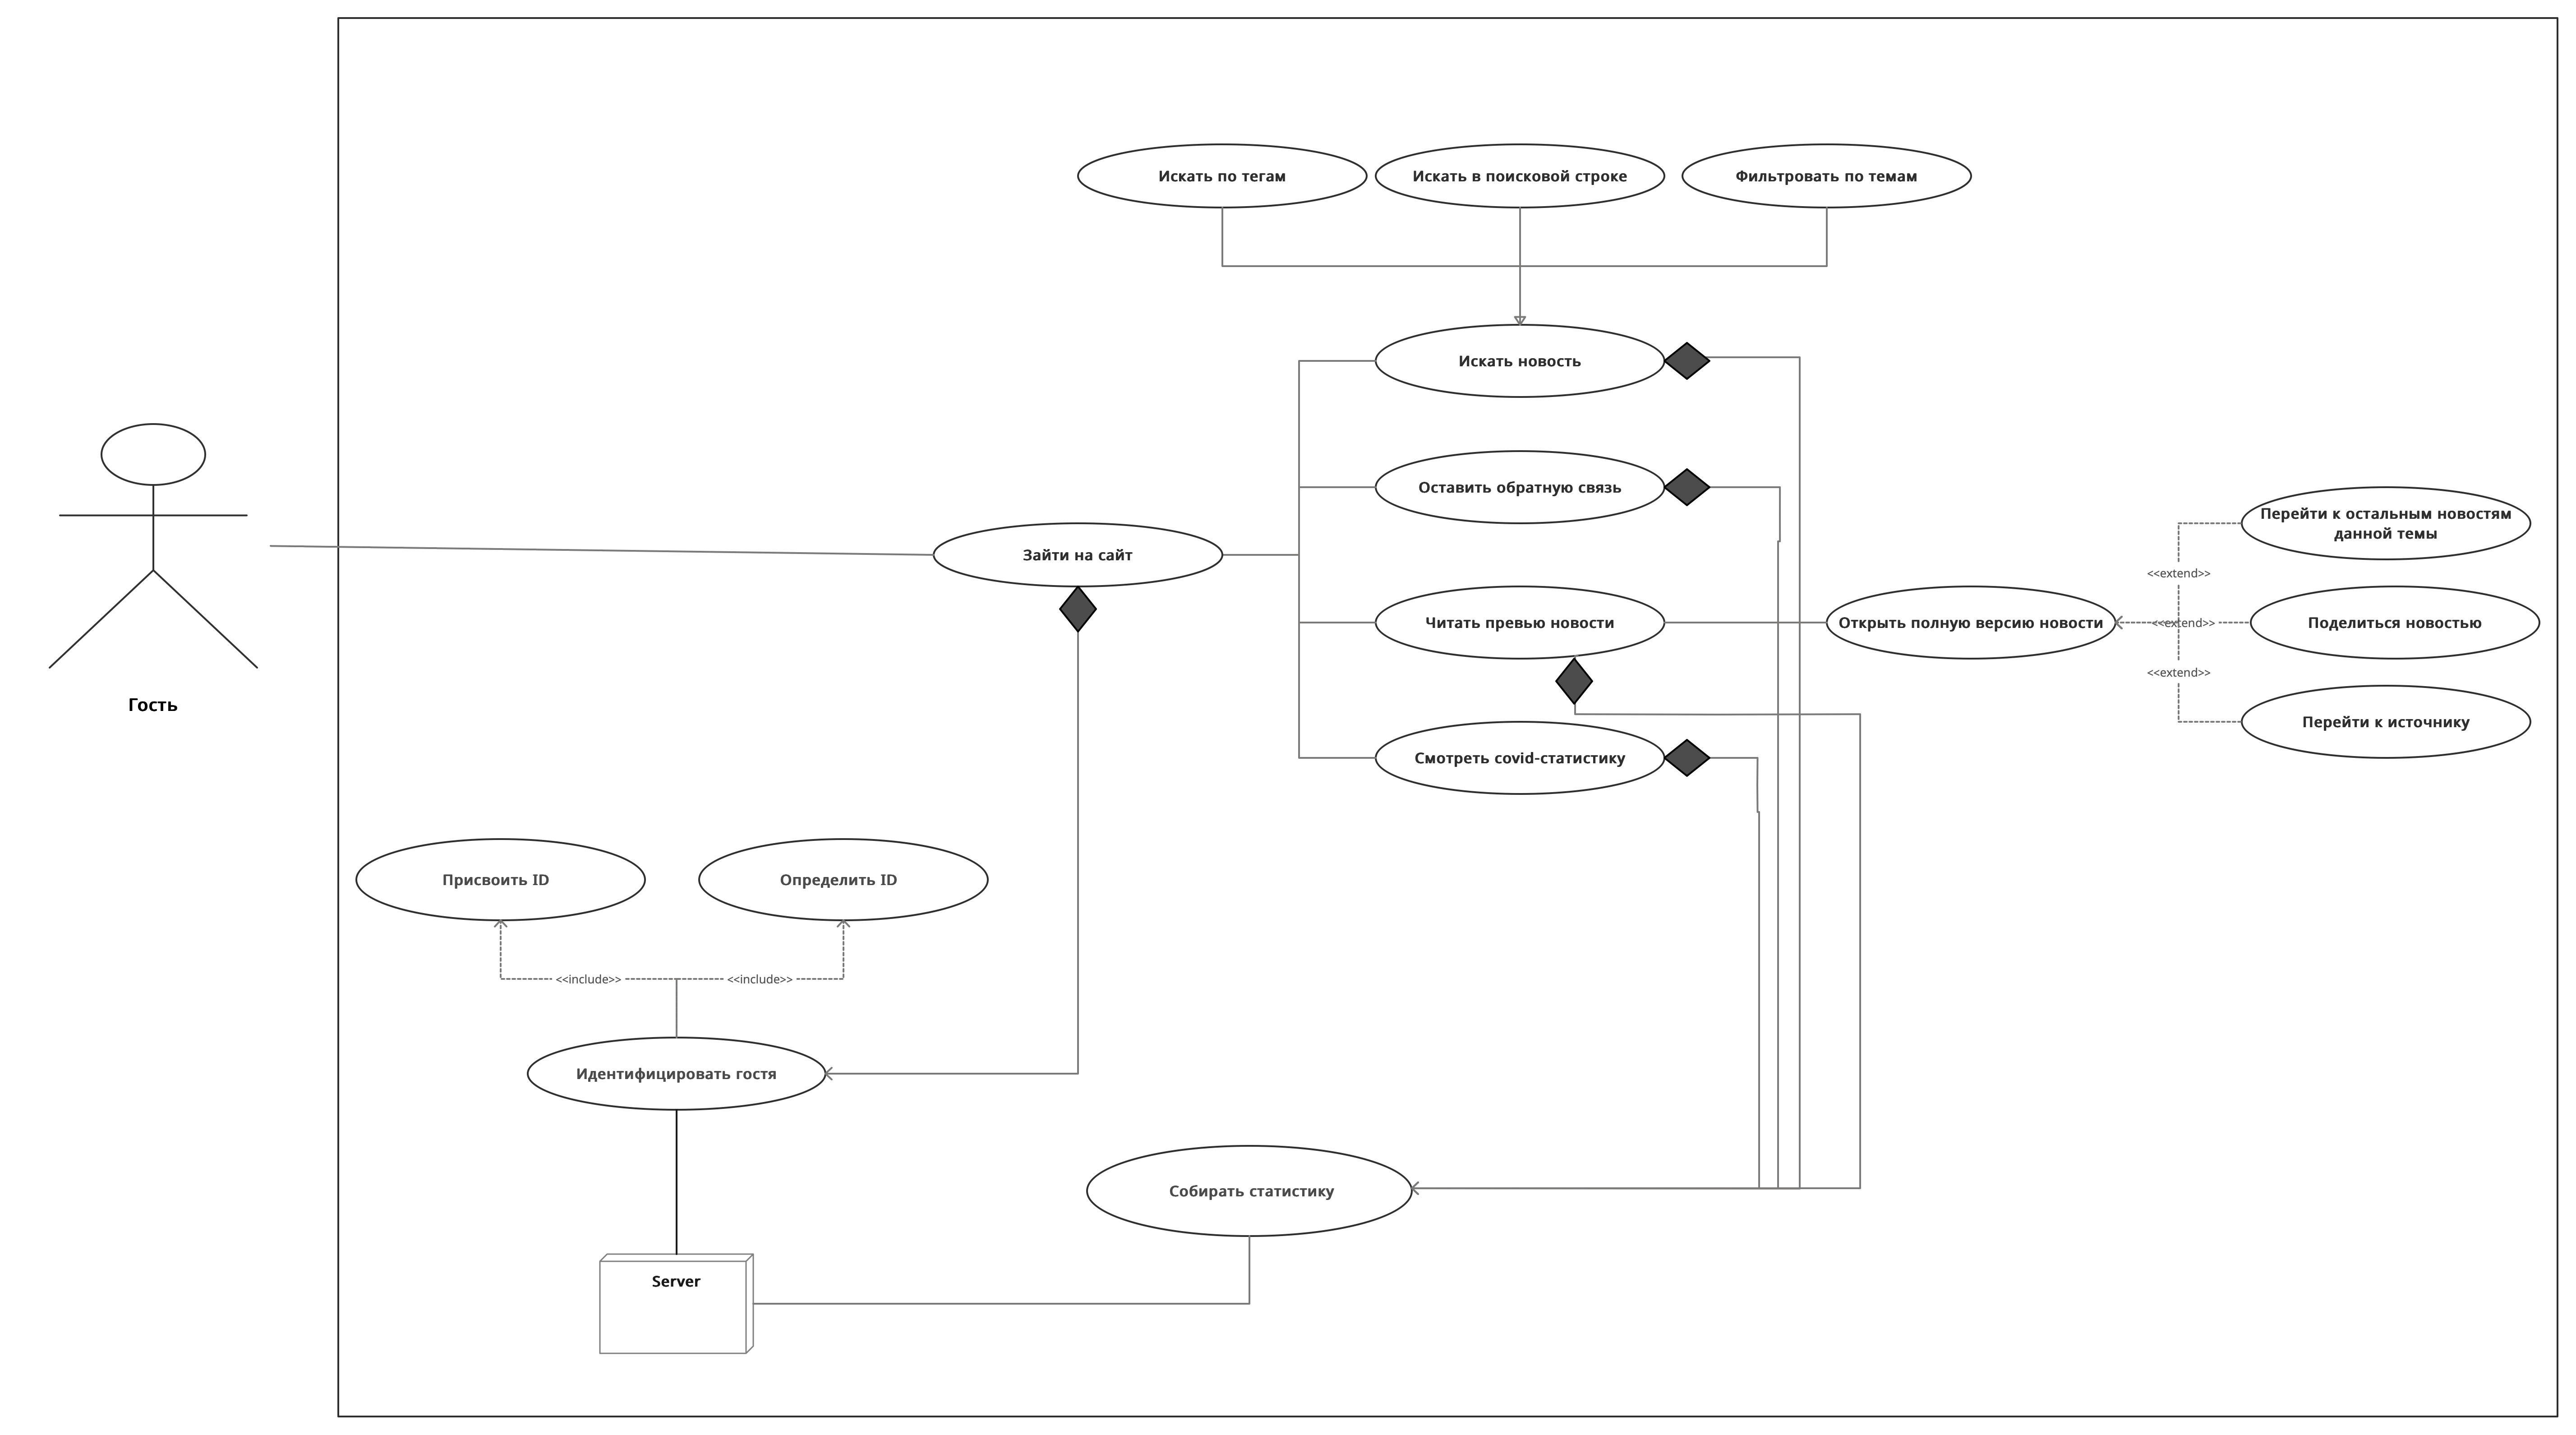
\includegraphics[scale=0.05]{img/Untitled Workspace-9}\\
        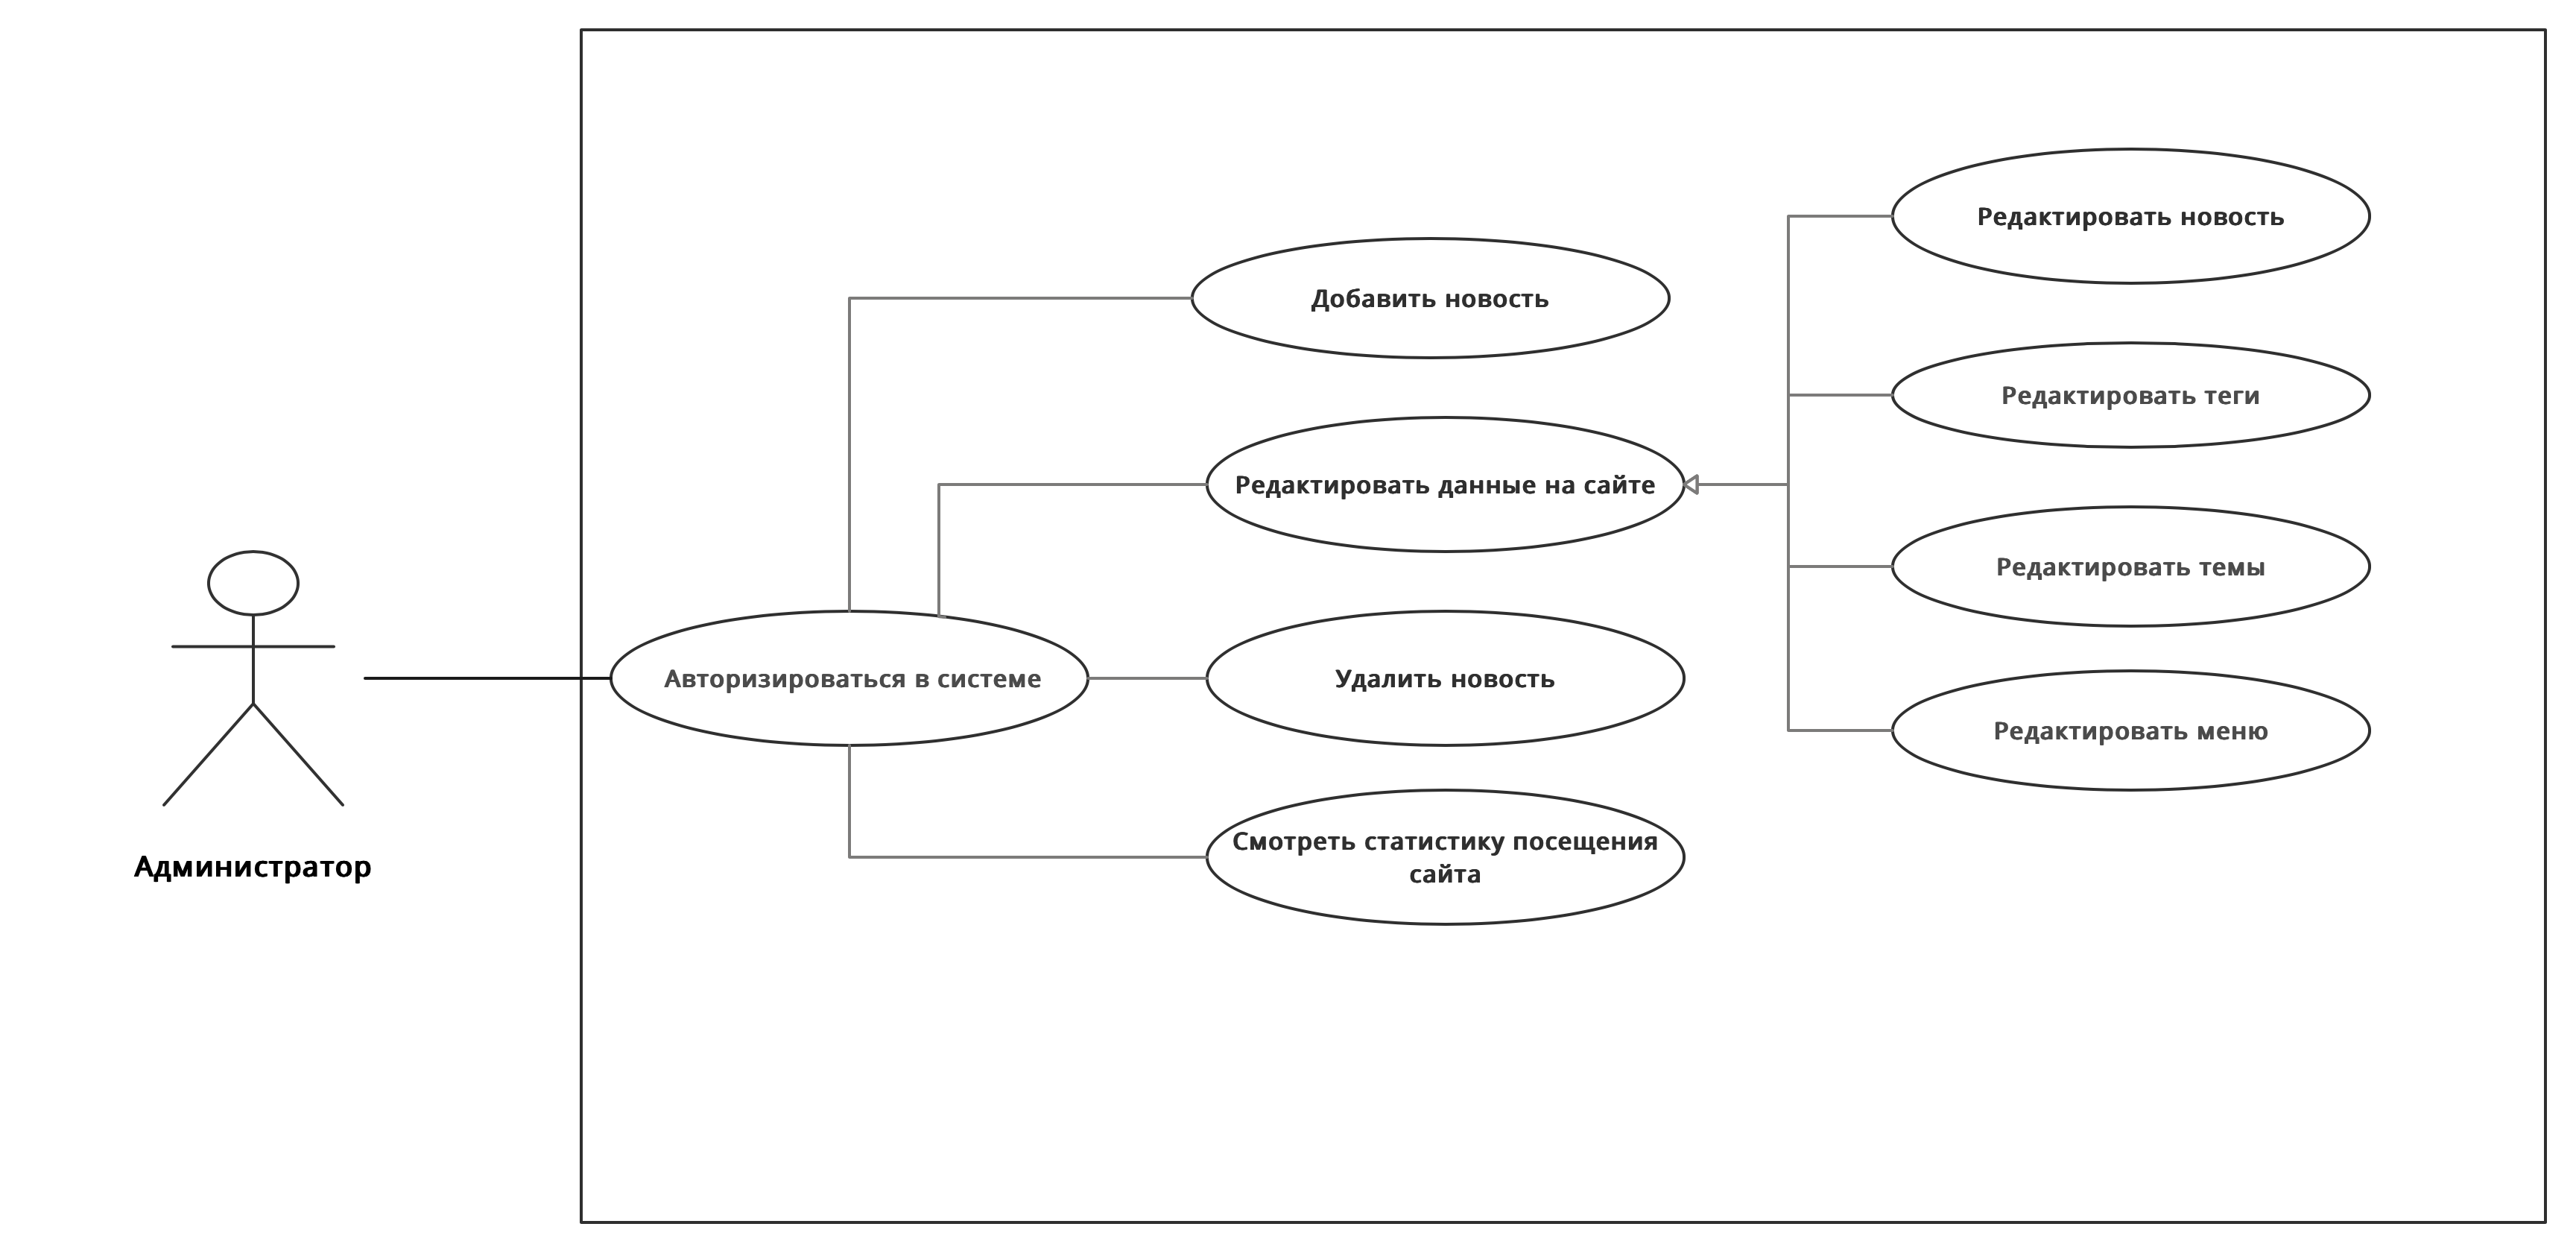
\includegraphics[scale=0.1]{img/Untitled Workspace-11}\\
    \end{figure}
\end{center}
\newpage
\BgThispage

\newpage
\BgThispage
\begin{center}
    \begin{figure}[H]
        \centering
        \includegraphics[scale=0.2]{img/Untitled}
    \end{figure}
    \begin{figure}[H]
        \centering
        \includegraphics[scale=0.15]{img/my_photo}
        \includegraphics[scale=0.225]{img/dora}
    \end{figure}
\end{center}